\documentclass[10pt]{beamer}

\mode<presentation> {

% The Beamer class comes with a number of default slide themes
% which change the colors and layouts of slides. Below this is a list
% of all the themes, uncomment each in turn to see what they look like.

%\usetheme{default}
%\usetheme{AnnArbor}
%\usetheme{Antibes}
%\usetheme{Bergen}
%\usetheme{Berkeley}
%\usetheme{Berlin}
%\usetheme{Boadilla}
%\usetheme{CambridgeUS}
%\usetheme{Copenhagen}
%\usetheme{Darmstadt}
%\usetheme{Dresden}
%\usetheme{Frankfurt}
%\usetheme{Goettingen}
%\usetheme{Hannover}
%\usetheme{Ilmenau}
%\usetheme{JuanLesPins}
%\usetheme{Luebeck}
%\usetheme{Madrid}
%\usetheme{Malmoe}
%\usetheme{Marburg}
%\usetheme{Montpellier}
%\usetheme{PaloAlto}
%\usetheme{Pittsburgh}
\usetheme{Rochester}
%\usetheme{Singapore}
%\usetheme{Szeged}
%\usetheme{Warsaw}

% As well as themes, the Beamer class has a number of color themes
% for any slide theme. Uncomment each of these in turn to see how it
% changes the colors of your current slide theme.

%\usecolortheme{albatross}
%\usecolortheme{beaver}
%\usecolortheme{beetle}
%\usecolortheme{crane}
\usecolortheme{dolphin}
%\usecolortheme{dove}
%\usecolortheme{fly}
%\usecolortheme{lily}
%\usecolortheme{orchid}
%\usecolortheme{rose}
%\usecolortheme{seagull}
%\usecolortheme{seahorse}
%\usecolortheme{whale}
%\usecolortheme{wolverine}

%\setbeamertemplate{footline} % To remove the footer line in all slides uncomment this line
\setbeamertemplate{footline}[page number] % To replace the footer line in all slides with a simple slide count uncomment this line

\setbeamertemplate{navigation symbols}{} % To remove the navigation symbols from the bottom of all slides uncomment this line
}

\usepackage{graphicx} % Allows including images
\usepackage{booktabs} % Allows the use of \toprule, \midrule and \bottomrule in tables
\usepackage{listings}

\title[DDP]{Attack on ROB and Prefetcher} % The short title appears at the bottom of every slide, the full title is only on the title page

\author{Meet Udeshi, Nirmal Boran\\
Prof. Virendra Singh} % Your name
\institute[CADSL] % Your institution as it will appear on the bottom of every slide, may be shorthand to save space
{
CADSL - IIT Bombay\\ % Your institution for the title page
}
\date{\today} % Date, can be changed to a custom date

\begin{document}

\begin{frame}
    \titlepage % Print the title page as the first slide
\end{frame}

\begin{frame}{Disabling Prefetcher to avoid Cache Pollution}
    \begin{itemize}
        \item Cache side-channels work by extracting information about cache accesses of victim process
        \item Any other process or hardware block which accesses the cache will increase noise in the side-channel
        \item Fuchs et al. \footnote{Disruptive prefetching: impact on side-channel attacks and cache designs - SYSTOR'15} have proposed a method to make prefetcher increase noise in cache and disrupt cache side-channel attacks
        \item We propose to disable the prefetcher by not allowing it to learn the stride patterns
        \item This can be done by running a third process in parallel which makes random loads at PC which alias with victim process' load PCs
    \end{itemize}
\end{frame}

\begin{frame}{Prefetcher attack implementation}
    \begin{itemize}
        \item Place load instructions at multiple PC address to fill up the prefetcher table
        \item Randomize stride for every load address
        \item Restrict load address to single cache line by keeping stride less than 64 bytes
        \item Ensure cache miss every time by flushing before load using \texttt{clflush}
        \item Use \texttt{nop} instructions to align loads to desired PC address
        \vspace{2em}
        \item Drawback: targets whole prefetcher and not few entries of victim
    \end{itemize}
\end{frame}

\begin{frame}[fragile]{Prefetcher attack implementation}
    \begin{lstlisting}
00000000000006ca <attack>:
 6ce:   8b 58 36        mov    0x36(%rax),%ebx
 6d1:   90              nop
 6d2:   0f ae 78 36     clflush 0x36(%rax)
 6d6:   8b 58 08        mov    0x8(%rax),%ebx
 6d9:   90              nop
 6da:   0f ae 78 08     clflush 0x8(%rax)
 6de:   8b 58 3f        mov    0x3f(%rax),%ebx
 6e1:   90              nop
 6e2:   0f ae 78 3f     clflush 0x3f(%rax)
 6e6:   8b 58 38        mov    0x38(%rax),%ebx
 6e9:   90              nop
 6ea:   0f ae 78 38     clflush 0x38(%rax)
 6ee:   8b 58 20        mov    0x20(%rax),%ebx
 6f1:   90              nop
    \end{lstlisting}
\end{frame}

\begin{frame}{Simulation setup}
    \begin{itemize}
        \item Simulator: gem5 X86
        \item Cores: 2
        \item L1: 32K icache 32K dcache private to each core
        \item L2: 256K 16-way shared between cores
        \item L2prefetcher: Stride 64-entry 4-way, confidence threshold 4
        \vspace{2em}
        \item Victim process runs on core1 and attacker runs on core2
        \item Number of prefetches issued are measured for every 100,000 instructions of victim process
    \end{itemize}
\end{frame}

\begin{frame}{Result plots: Number of prefetches}
    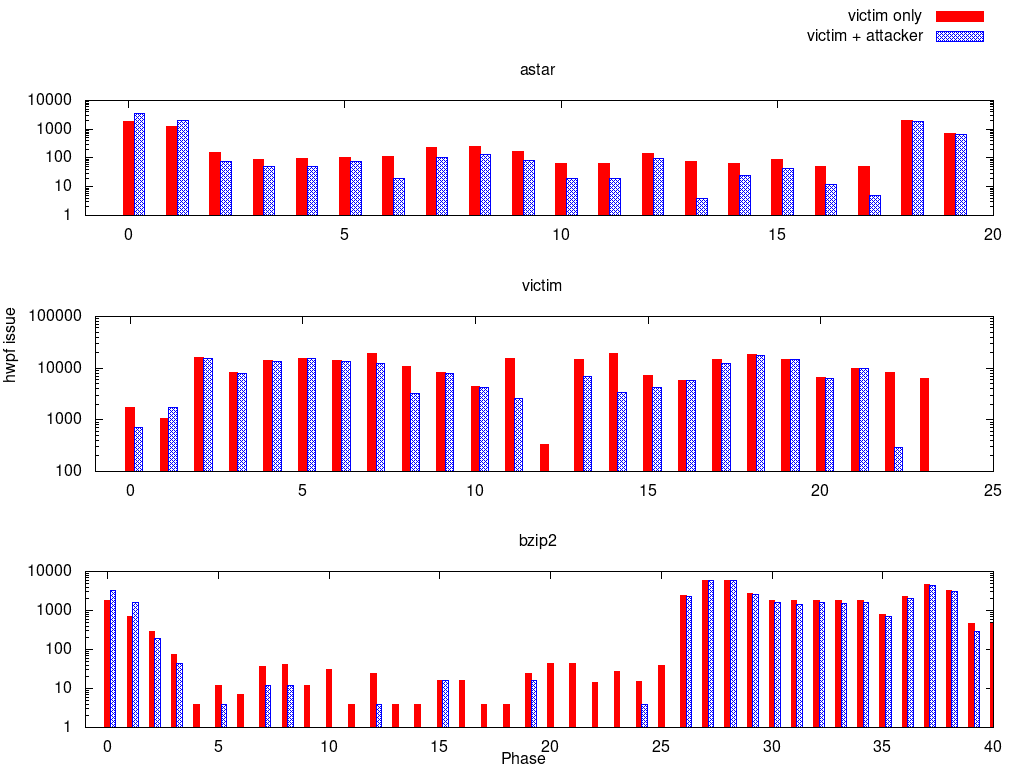
\includegraphics[width=0.95\textwidth]{hwpf_num.png}
\end{frame}
\begin{frame}{Result plots: Percent reduction}
    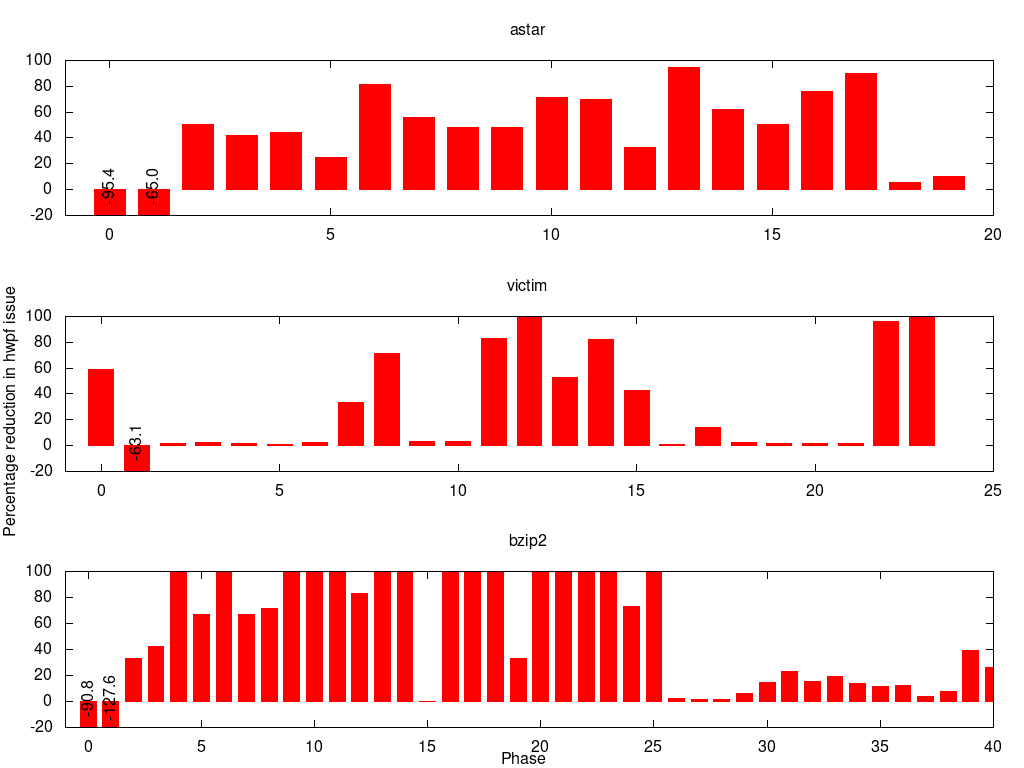
\includegraphics[width=0.95\textwidth]{hwpf_perc.png}
\end{frame}

\begin{frame}{Future work}
    \begin{itemize}
        \item Analyse why prefetches are not reducing to 0
        \item Devise attack tailored to victim's loads
        \item Try with openssl AES code
    \end{itemize}
\end{frame}

\begin{frame}
    \Huge{\centerline{The End}}
\end{frame}

\end{document}